\title{Classes of Inference}

{{navbar}}

\subsubsection{Classes of Inference}

Edward uses class inheritance to provide a hierarchy of inference
methods. Inference is broadly classified under three components:
variational inference, Monte Carlo, and exact inference.

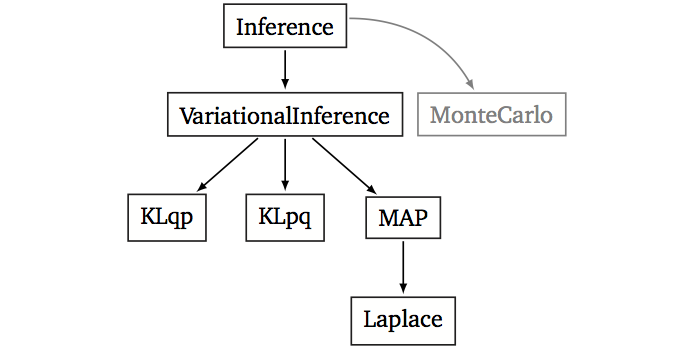
\includegraphics[width=700px]{/images/inference_structure.png}
{\small\textit{Dependency graph of inference methods.
Nodes are classes in Edward and arrows represent class inheritance.}}

Below we highlight how to use inference algorithms from each class.

\subsubsection{Variational Inference}

% In general, Edward takes a variational perspective of inference, where
% there is always an approximating family. Inference is about matching
% the approximating family to the posterior.

Variational inference approximates the posterior by solving an
optimization problem.  We define the variational family and match its
factors to latent variables in the model according to this
optimization.
\begin{lstlisting}[language=Python]
qbeta = Normal(mu=tf.Variable(tf.zeros([d])),
               sigma=tf.nn.softplus(tf.Variable(tf.ones[d])))
qz = Normal(mu=tf.Variable(tf.zeros([d])),
            sigma=tf.nn.softplus(tf.Variable(tf.ones[d])))

inference = ed.VariationalInference({beta: qbeta, z: qz}, data={x: x_train})
\end{lstlisting}
Given an objective function, variational inference optimizes the
factors with respect to \texttt{tf.Variable}s.

Maximum a posteriori (MAP) approximates the posterior using the mode.
In Edward, we view MAP as a form of variational
inference where the approximating family is a point mass distribution,
i.e., a distribution with all probability mass concentrated at a
point.
\begin{lstlisting}[language=Python]
qbeta = PointMass(params=tf.Variable(tf.zeros([d])))
qz = PointMass(params=tf.Variable(tf.zeros([d])))

inference = ed.MAP({beta: qbeta, z: qz}, data={x: x_train})
\end{lstlisting}

\subsubsection{Monte Carlo}

Monte Carlo approximates the posterior using samples. In Edward, we view
Monte Carlo as a form of inference where the approximating family is
an empirical distribution.
\begin{lstlisting}[language=Python]
T = int(1e4)  # number of samples
qbeta = Empirical(params=tf.Variable(tf.zeros([T, d]))
qz = Empirical(params=tf.variable(tf.zeros([T, d]))

inference = ed.MonteCarlo({beta: qbeta, z: qz}, data={x: x_train})
\end{lstlisting}
Monte Carlo proceeds to update the \texttt{tf.Variable}s one sample
at a time. Markov chain Monte Carlo does this sequentially to update
the current sample (index $t$ of \texttt{tf.Variable}s) conditional on
the last sample (index $t-1$ of the \texttt{tf.Variable}s).

\subsubsection{Exact Inference}

Edward also supports exact inference.

Collapsing discrete random variables.
TODO has to explicitly define distribution form
TODO this is a special case of the marginal below; maybe then we can organize these two as tractable marginals and tractable posteriors? (depends on if conjugacy also means tractable marginals)
\begin{lstlisting}[language=Python]
z = Categorical(logits=tf.random_normal([K]))
x = Normal(mu=tf.gather(mus, z), sigma=tf.gather(sigmas, z))

cat = Categorical(logits=tf.Variable(tf.random_normal([K])))
components = [Normal(mu=tf.Variable(tf.random_normal([D])),
                     sigma=tf.Variable(tf.random_normal([D])))
              for _ in K]
qx = Mixture(cat=cat, components=components)

inference = CollapsedInference({x: qx})
inference.run()
\end{lstlisting}

Conjugate inference. It can be used for calculating both tractable posteriors and tractable marginal densities.
TODO has to explicitly define distribution form
\begin{lstlisting}[language=Python]
z = Gamma(alpha=tf.constant([1]), beta=tf.constant([1./2]))
x = Exponential(lam=z)

qx = Gamma(alpha=tf.Variable(tf.random_normal([1])),
           beta=tf.Variable(tf.random_normal([1])))

inference = ConjugateInference({x: qx})
inference.run()
\end{lstlisting}

Symbolic inference.
TODO has to explicitly define distribution form of posterior
functions of rvs
\begin{lstlisting}[language=Python]
eps = Normal(mu=tf.constant([0.0]), sigma=tf.constant([1.0]))
x = mu + sigma * eps

qx = Normal(mu=tf.Variable(tf.random_normal([1])),
            sigma=tf.Variable(tf.random_normal([1])))

# using, e.g., Maple
inference = SymbolicInference({x: qx})
inference.run()
\end{lstlisting}

(we can also do deterministic approximations; not sure what's a better subsection to this)

Numerical integration. This includes for example Riemannian sums, Gaussian quadrature,
adaptive quadrature, and quasi-Monte Carlo.
\begin{lstlisting}[language=Python]
x = Normal(0, 1)
fx = f(x)
# TODO how to represent E_{p(x)} [ f(x) ]?

output = tf.Variable(tf.random_normal(1))

# We want E_{p(x)} [ f(x) ].
inference = GaussianQuadrature({ : output}))
inference.run()
\end{lstlisting}

{{autogenerated}}
